\documentclass[a4paper,12pt]{article} 
\usepackage[T1]{fontenc} 
\usepackage{enumerate}
\usepackage{enumitem}
\usepackage{graphicx}
\usepackage{listings}
\usepackage{wrapfig}
\usepackage{subfigure}
\usepackage[a4paper,top=2.5cm,bottom=2.5cm,left=2.5cm,right=2.5cm]{geometry}
\usepackage{array}
\usepackage{tablefootnote}
\usepackage{float}
\setlength\extrarowheight{2pt}

\title{\bf Clustering of handwritten words based on structural features extraction}
\date {17 February 2015}
\author{Lorenzo Cioni, Francesco Santoni\\\textit{{\small lore.cioni@gmail.com, fsanto92@hotmail.it}}}

\begin{document}
\maketitle

\begin{abstract}

In this report we discuss our application for the extraction of primitive features from images of handwritten words and the generation of clusters of similar elements. In this case the words, compared to the names of American States and other countries, are extracted from forms of the 1930' U.S. census.
\end{abstract}

\tableofcontents

\section{Introduction}
Segmentation and clustering of large amounts of data is one of the main research fields of modern artificial intelligence.

The basis of our work is the collection of u.s. Census data in the year 1940 and fits into the process of digitalizing of handwritten documents that characterizes our time. In this case we have scans of census register and the main problem is to divide enrollees for each American State.

Document segmentation and extraction of the word corresponding to the State was developed previously by two of our colleagues in the course of \emph{Technology of Databases} and is the base from which our work started.So the problem on which we have worked is the extraction of features from handwritten characters to cluster similar words in order to facilitate the recognition by a human agent.

\begin{figure}[!ht]
\centering
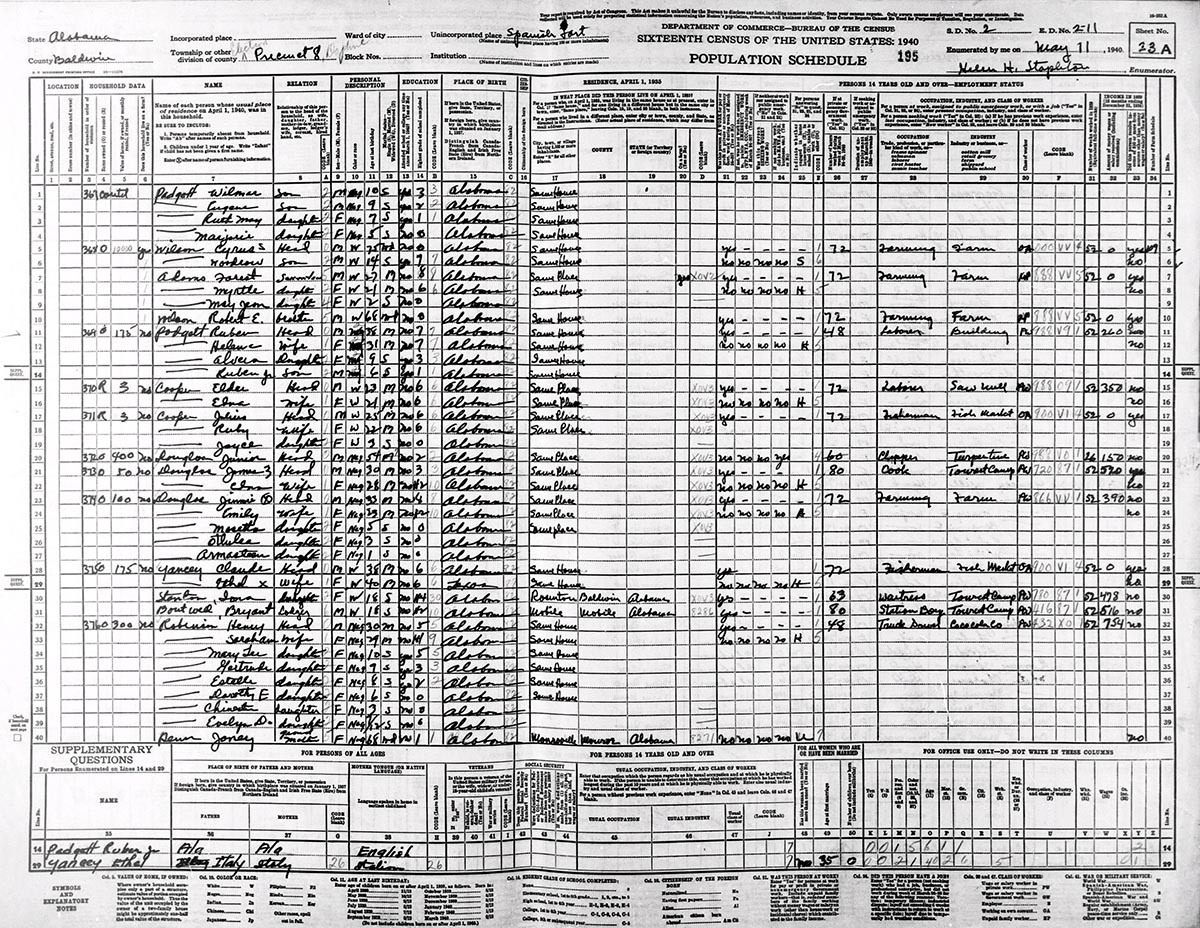
\includegraphics[width=0.6\textwidth]{images/img1.jpg}
\caption{An example of a table containing census data}
\end{figure}
\section{The pre-existing project}

The census page that contains the data in digital form holds a wealth of information about each person surveyed: name, gender, membership status and some secondary features such as work or the breed. 

All these data are housed in a moulded grid composed of numbered rows and columns. In addition to the citizens data, each archive also contains additional information related to the censor or data relating to samples of the population.

The project's objective was finding a particular grid area, corresponding to the area containing the registered State of each person, from which extract the handwritten text.

Following the words localization, the existing work proceeds by grouping visually similar elements to form a collection of homogeneous samples, in hope that each set will then contain cut outs of the same State.

The goal of the work is not to group all the words corresponding to the same state in a single cluster but rather to generate clusters that contain words that belong to a single state, the major requirement of the work is thus precision in the retrieval steps.

\subsection{Process steps}

We can summarize the project in three basic steps:
\begin{enumerate}
\item Localization of the text area containing the words of interest
\item Row segmentation
\item Post-processing and clustering
\end{enumerate}

The last step, corresponding to the clustering of images, is the point of interest of our paper: while the past work was focused on the localization and retrieval not much thought was put on the features to be extracted preferring simplicity and efficiency to effectiveness.
It is this very point that gives our paper a reason d'etre: starting from the preceding, already implemented, two steps, we proceed by providing a rewritten and improved clustering method through the use of new features, these steps will be discussed later in the section 3.

\subsubsection{Column localization}

In this first phase the aim is to identify the region of the grid within which the State words are located. 

First of all the black border of the document is removed, an artefact resulting from the physical scanning. Then, through a vertical projection of the pixels and the creation of an histogram, the grid columns are located and, knowing the correct column's offset regarding the beginning of the document, just the one concerned is extracted.

\subsubsection{Row segmentation}

After the extraction of the concerned column from the document, we proceed with row segmentation.

Similar to the previous step, but using an horizontal projection this time, we are able to determine with some accuracy the rows of the grid. In this case, however, it's necessary to centre the word in the extracted image: this is done by correcting the height of each row by the analysis of black spikes on the created histogram.

At the end of this phase, ideally each word is contained in an individual image.

\subsubsection{Post-processing and clustering}

In the post-processing phase the individual images extracted are reworked in order to remove any  vertical or horizontal residual lines left from an imperfect previous cut.

Delete row/column strokes can be about as bring back the black pixels related to the residual value of pure white (255 as grayscale).

This allows us to extract the most significant features in the next steps of processing.

Each image is divided in windows 1 pixel wide, on these windows the features are then extracted.
The idea is not placing excessive burden on the operating system, the features are thus relatively simplistic: for each window the value of the height of the first and last black pixels are collected, together with the number of transitions of the pixels from black to white and vice versa.
The distance between images is then found through the Euclidean Distance where the considered axis are the number of transitions and the stroke height calculated through a simple subtraction of the first and last black pixels height.
The distance matrix is then fed to the Affinity Propagation algorithm to create the desired clusters.

\begin{figure}[!ht]
\centering
\vspace{0.3cm}
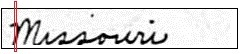
\includegraphics[width=0.5\textwidth]{images/missouri_1pix.jpg}
\caption{An image extracted from document, the red box delineates the 1 pixel wide window.}
\label{fig:extracted_image}
\end{figure}

As you can see in Figure \ref{fig:extracted_image}, the word is centered and the extra line have been removed (there is a line set to white). For each picture we proceed with feature extraction for handwritten characters and clustering. 

\subsection{Problems}

The localization of words and their segmentation has inherent strong difficulties.

A first problem is represented by the document skew. In this case, the skew may be due to a not perfectly horizontal scan of the original document. The presence of skew reduces the capability in searching for rows and columns of the grid, thus making the segmentation impossible with the given implementation. In some cases, for example, the first column is interpreted incorrectly causing the extraction of the wrong column in the first stage of the process thus dooming that particular word recognition.

The main problems of the second phase are mainly related to the identification of extraneous lines. Because of the large number of dashed lines present it isn't always possible to \emph{clean} the images and this can cause errors in the clustering phase.

\begin{figure}[!ht]
 \centering
 \subfigure[An image with a dashed line]
   {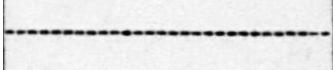
\includegraphics[width=0.3\textwidth]{images/img3.jpg}}
 \hspace{5mm}
 \subfigure[The line intersects the word]
   {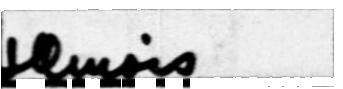
\includegraphics[width=0.3\textwidth]{images/img4.jpg}}
 \caption{Segmentation and post-processing issues}
 \end{figure}

In other cases the word intersects directly gridlines. Because of this we may experience a loss of information about words if the line is removed using the method described above.


\section{Features extraction}

\subsection{Structural features}

In this work we want to find \emph{primitive} features, resembling the possible types of strokes used to write a word, to characterize the sample from which they are extracted in order to perform clustering on their set.

The features are identified by the study of a sub-portion, or window, of the images extracted by the paper on which this work is based.

The features are located through a study of an area, the window, with which they are implicitly associated: as such there is no clear order of which of the possibly multiple features found in the area comes first.
Due to the absence of such \emph{native} order the string that defines a window is maintained consistent with the other strings trough the convention of generating the string with the features' identifiers always taking the same order, if present.

The chosen way to resolve the issue however presents the problem of making sliding windows inapplicable: this means that a sample must necessarily be cut in separate windows, which are allowed to overlap, with the corresponding effect that due to the random cut some features like \textit{loops} may not be recognised in an instance and recognised in another. 

Each sample is associated to a characterizing string of characters made from the identifiers of the features recognized in the sample.

The string is constructed modularly by appending in order the strings associated to each window the sample is divided in.

After having recognised the presence of a feature in a given window the corresponding identifier is added to the end of the string correspondent to the window; the order in which the features are searched and thus added to the queue is decided a priori and maintained consistent during the construction of the strings. 


\paragraph{Windows}

Currently we have chosen to cut the samples in windows of 32 pixels each, with the exception of the last part of the sample that, deemed irrelevant to the end of characterization due to containing almost always white space, is simply ignored.

These windows are spaced only 16 pixels from the preceding and succeeding one, with the intent of creating overlap and lengthening the string that characterizes the samples.

While the simplest way to create the windows is simply creating a new PIX with the required coordinates it requires unnecessary passages and time in the creation of new objects. We have thus preferred to increase the complexity of the functions that search for the features, to whom we pass as a variable the original sample PIX with information about the \textit{offset} at which to start the search and the \textit{width} of the window. The width of the window passed has actually a non banal meaning duo to the fact that different features are linked to areas of the image with varying dimensions: for example we can't reasonably search for an horizontal line and a vertical line utilizing windows with the same width due to the fact that horizontal lines realistically will require windows with great width but will not have requisites on the height.

The height of the windows used is never considered as a parameter since for all features' functions the height is customarily the whole height of the sample.  

\subsubsection{Whitespace}  

The first feature that is search in the windows is the white space. This way if a window is identified as blank will not be necessary to proceed with the investigation of other features, saving time.

\begin{figure}[!ht]
\centering
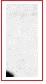
\includegraphics[width=0.06\textwidth]{images/whitespace.jpg}
\caption{A whitespace}
\end{figure} 

A window is identified as blank if the average pixel values is below a preset white threshold.

\subsubsection{Loop}

The feature that represents a loop is recognized only with maximum window size.
To locate a loop is initially found a black pixel. The idea behind is to imagine that we had found a point on the border and meet two transitions going in the same direction, first from black to white then from white to black. Between the two transitions there must be a minimum step above a preset threshold where the pixels are white.

\begin{wrapfigure}{l}{0.3\textwidth}
  \vspace{-20pt}
  \begin{center}
    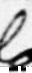
\includegraphics[width=0.06\textwidth]{images/loop.jpg}
  \end{center}
  \vspace{-20pt}
  \caption{A loop}
  \vspace{-10pt}
\end{wrapfigure}

If the above condition occurs then we verify that it is real in the same way along the horizontal axis. We then sit in the center of the loop (the median value of the segment described above) and check that, moving both right or left you get a transition from white to black after a suitable number of white pixels.

The implemented method has numerous problems related mainly to the identification of the center of the loop in the segment. With a value of threshold too high also might have to discard some loops too small. The method also does not take into account the thickness of the stroke.
However, with appropriate threshold values you can get good results and to identify obvious loops of various segments.

\subsubsection{Dot}

\begin{wrapfigure}{r}{0.3\textwidth}
  \vspace{-20pt}
  \begin{center}
    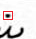
\includegraphics[width=0.06\textwidth]{images/dot}
  \end{center}
  \vspace{-20pt}
  \caption{A dot}
  \vspace{-10pt}
\end{wrapfigure}

To search for Dots within the segment we first proceed locating the \emph{connected components} inside it. The individual components are extracted and inserted into a \emph{box} which we can know the size and the relative position to the segment.


At this point we look for those boxes with dimensions between two preset values (minimum and maximum radius) and those that meet this condition are most likely points.

Using connected components we can retrieve Dot feature in a simple way.

\subsubsection{Diagonal line}

The feature representing a diagonal line, both upward and downward facing, is extracted through a simple exhaustive scansion of the window for lines of connected black pixels that have an incline in a range of values and are sufficiently long.

At the moment the function doesn't account for the width of the lines found, thus diagonal features can be recognised in a shapeless blob of black pixel that is sufficiently big. 
\begin{wrapfigure}{l}{0.3\textwidth}
  \vspace{-20pt}
  \begin{center}
    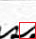
\includegraphics[width=0.06\textwidth]{images/diagonal.jpg}
  \end{center}
  \vspace{-20pt}
  \caption{A diagonal line}
  \vspace{-10pt}
\end{wrapfigure}
   
There's a distinction for diagonal features that appear in the lower and upper bottom of the window.
At most in a window the function identifies a couple of upward and a couple of downward facing lines (lower and upper parts), once one has been found it stops searching for the same type.

\subsubsection{Cross}
The function, having found at most a lower and upper case for upward and downward diagonal lines, proceeds to confront the edge points of these lines: if they possibly intersects it extracts a \emph{crossing} feature with distinction if the crossing happens in the lower or upper part of the window. 

The problems with this sub-feature are that intersections of bottom and upper lines of the same type (e.g. both upward facing) with different inclines are not recognised, in the same way there's no consideration for intersections made from lines that are not the "primary" bottom and upper diagonals: if in a single windows are present more lower upwards diagonals and one of them other than the first intersects the recognised downward diagonal, such a crossing is ignored.

The crossing feature may also not necessarily be a complete intersection, in fact for recognition there just needs to be a merging of a downward and upward line. 


\subsubsection{Horizontal and Vertical line}
Both horizontal and vertical lines' features are extracted through
a simple scan of the window.

The horizontal lines requires a double-window for their implicit characteristic.
The function identifies a line if it finds a connected row or column of black pixels that has sufficient length, in particular it distinguishes the lines found in normal or long through an ulterior threshold.

Once a fitting line has been found the function keeps searching for more, continuing the scansion of the window after having moved a certain distance from the last line found in order not to confuse a particularly thick stroke as different separate lines.

There still persists the problem that the stroke width is not fully considered so a big blob of black pixels is seen as a series of horizontal and vertical lines, at the same time such an occurrence is rare so the presence of many horizontal and vertical lines ends up distinguishing the word in itself.    

\subsection{Dimensional features}

In some cases the structure feature extraction leads to some problems of recognition or it may not be sufficient to properly assess the similarity between two words.

In order to improve word clustering we combine structural features with \emph{dimensional features} for each word. 

As in the previous feature extraction process, words are splitted in smaller boxes. For each of them we evaluate the stroke height and the number of transitions from white to black. With those features two words are similar if their strokes are similar compared by length and height. The height is stored as the difference between the end of the stroke and the start.

\subsection{Features extraction example}

We present now an example of extraction of features from a word. We initially create, as described above, a sliding window that scrolls along the image by a fixed step. Than, for each section,  features are extracted and a substring is generated.

\begin{figure}[!ht]
\centering
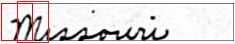
\includegraphics[width=0.5\textwidth]{images/missouri_crop.jpg}
\caption{Feature extraction from \emph{Missouri} word}
\end{figure} 

\begin{figure}[!ht]
 \centering
 \subfigure[]
   {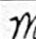
\includegraphics[width=0.06\textwidth]{images/missouri/0.jpg}}
 \subfigure[]
   {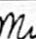
\includegraphics[width=0.06\textwidth]{images/missouri/1.jpg}}
 \subfigure[]
   {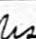
\includegraphics[width=0.06\textwidth]{images/missouri/2.jpg}}
 \subfigure[]
   {
\includegraphics[width=0.06\textwidth]{images/missouri/3.jpg}}
 \subfigure[]
   {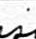
\includegraphics[width=0.06\textwidth]{images/missouri/4.jpg}}
 \subfigure[]
   {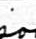
\includegraphics[width=0.06\textwidth]{images/missouri/5.jpg}}
 \subfigure[]
   {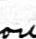
\includegraphics[width=0.06\textwidth]{images/missouri/6.jpg}}
 \subfigure[]
   {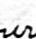
\includegraphics[width=0.06\textwidth]{images/missouri/7.jpg}}
 \subfigure[]
   {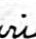
\includegraphics[width=0.06\textwidth]{images/missouri/8.jpg}}  
 \subfigure[]
   {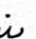
\includegraphics[width=0.06\textwidth]{images/missouri/9.jpg}}
 \subfigure[]
   {
\includegraphics[width=0.06\textwidth]{images/missouri/10.jpg}}
 \subfigure[]
   {
\includegraphics[width=0.06\textwidth]{images/missouri/11.png}}
 \subfigure[]
   {
\includegraphics[width=0.06\textwidth]{images/missouri/12.png}}   
 \caption{Sliding window segmentation}
 \end{figure}

\begin{enumerate}[label=(\alph*)]
\item Some \textbf{diagonal lines} (ascending (s) and descending (u) ), at the top (S) and at the bottom (s) of the image. Generated string: ''\emph{sSUusSUSu}''.
\begin{figure}[!ht]
\centering
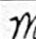
\includegraphics[width=0.06\textwidth]{images/missouri/0.jpg}
\end{figure} 
\item As the previous image and two more diagonal lines representing the "\emph{i}". An \textbf{horizonal line} (H). Generated string: ''\emph{sSUusSUSuHsu}''.
\begin{figure}[!ht]
\centering
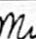
\includegraphics[width=0.06\textwidth]{images/missouri/1.jpg}
\end{figure} 
\item Some diagonal lines and, at the end of the window, an horizontal line. Generated string: ''\emph{ssSusSsH}''.
\begin{figure}[!ht]
\centering
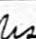
\includegraphics[width=0.06\textwidth]{images/missouri/2.jpg}
\end{figure} 
\item Two consecutive similar character represented by diagonal lines and \textbf{vertical lines} in the middle. Generated string: ''\emph{sVHsV}''.
\begin{figure}[!ht]
\centering

\includegraphics[width=0.06\textwidth]{images/missouri/3.jpg}
\end{figure} 
\item In that window we can find a \textbf{dot} (.). Generated string: ''\emph{ssVHs.}''
\begin{figure}[!ht]
\centering
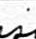
\includegraphics[width=0.06\textwidth]{images/missouri/4.jpg}
\end{figure} 
\item The same previous dot and a little \textbf{loop} (L) at the bottom. Generated string: ''\emph{ssVs.LssH}''.
\begin{figure}[!ht]
\centering
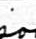
\includegraphics[width=0.06\textwidth]{images/missouri/5.jpg}
\end{figure} 
\item The same loop as previous, an horizontal line a vertical line and two diagonal. Generated string: ''\emph{LVHssu}''.
\begin{figure}[!ht]
\centering
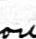
\includegraphics[width=0.06\textwidth]{images/missouri/6.jpg}
\end{figure} 
\item Generated string: ''\emph{ssVHus}''.
\begin{figure}[!ht]
\centering
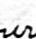
\includegraphics[width=0.06\textwidth]{images/missouri/7.jpg}
\end{figure} 
\item The other dot here. Generated string ''\emph{ssus.H}''.
\begin{figure}[!ht]
\centering
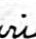
\includegraphics[width=0.06\textwidth]{images/missouri/8.jpg}
\end{figure} 
\item An i. Generated string: ''\emph{ssuu.}''.
\begin{figure}[!ht]
\centering
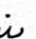
\includegraphics[width=0.06\textwidth]{images/missouri/9.jpg}
\end{figure} 
\item Only a diagonal line. Generated string: ''\emph{s}''.
\begin{figure}[!ht]
\centering

\includegraphics[width=0.06\textwidth]{images/missouri/10.jpg}
\end{figure} 
\item Empty window. Generated string: ''\emph{ }''.
\begin{figure}[!ht]
\centering

\includegraphics[width=0.06\textwidth]{images/missouri/11.png}
\end{figure} 
\item Empty window. Generated string: ''\emph{ }''.
\begin{figure}[!ht]
\centering

\includegraphics[width=0.06\textwidth]{images/missouri/12.png}
\end{figure} 
\end{enumerate}

Once those strings are generated they are combined together to generate the word \textit{structure string}. 


\subsection{Evaluating distances}

\subsubsection{Longest Common Subsequence} 

In order to compare the generated strings one another we must define a distance on the samples.
The distance used in our work is based on the \emph{Longest Common Subsequence} (\textbf{LCS}) algorithm. 

The LCS algorithm has the aim of extracting from a set of sequences (in this case only two) the longest common subsequence, that is a sequence that is obtainable from both the starting sequences by deleting some elements without changing the order of the remaining ones.

LCS is a particular case of the \emph{Edit Distance} algorithm where the only allowed operations are insertion and deletion.
The distance associated with LCS in our current work is the number of insertion and deletions that must be applied to obtain the longest subsequence, in accordance with the Edit distance where the distance is calculated with the number of operations needed to morph a string in the other (in Edit Distance it's possible moreover to confer customizable costs to the substitutions).   

While the LCS algorithm may require high costs when applied concurrently to high numbers of sequences, in our case there exists an easy and light implementation that exploits \textit{dynamic programming}, in this type of implementation the cost ends up being $O(n*m)$ where $n$ and $m$ are the length of the compared strings.  


$$\label{LCS}
LCS(X_i,Y_j) =
 \left\{\begin{array}{ll}
 \displaystyle
 0 & if~i=0~ or~ j=0\\
 LCS(X_{i-1},Y_{j-1})\cup x_i & if~ x_i=y_j\\
 longest(LCS(X_i,Y_{j-1}), LCS(X_{i-1},Y_j)) & if~ x_i\neq y_j
 \end{array}\right.
$$


Obtained the Longest Common Subsequence between two strings the distance between them is thus:
$$ x.length() + y.length() - 2*LcsLength$$

where $x$ and $y$ are the strings and the $length()$ function returns the length of a string.

\subsubsection{Euclidean distance} 

Longest Common Subsequence is only used with strings. In order to improve the correctness of words distance we combine LCS distance with euclidean distance which uses dimensional features insted of structure features.

The eucliden distance is evaluated with
$$d = \sqrt{((a_b - a_t)−(b_b - b_t))^2 +(a_c - b_c)^2}$$

with

\begin{itemize}
\item $a_b$ representing the end of the stroke $a$
\item $a_t$ representing the begin of the stroke $a$
\item $b_b$ representing the end of the stroke $b$
\item $b_t$ representing the begin of the stroke $b$
\item $a_c$ representing the number of transition (normalized) of $a$
\item $b_c$ representing the number of transition (normalized) of $b$
\end{itemize}

At this point we evaluate the L1 normalization for each segment we proceed evaluatin distances from different features with the previous way.
\section{Clustering}
\label{Nostro_prog}
The clustering phase consists in the categorization of the various segments in homogeneous groups, so that, at the end of the process, each cluster contains  words corresponding to the same State.

At this stage the main goal is the extraction of good features representative of the images to be used for comparison. The aim is to construct a similarity matrix between different segments so that they can be used as input to the clustering algorithm. To do so we generate a measure of distance between couples of samples through the use of the \emph{Longest Common Subsequence} algorithm in which the handled strings, representative of the corresponding samples, are constructed through the appending of conventional identifiers associated with the features found in the samples in a consistent order. 

Unable to establish a priori the optimal number of desired clusters makes the use of the \emph{Affinity Propagation} algorithm a necessity.

\subsection{Affinity Propagation}

Affinity Propagation is a clustering algorithm that identifies a set of \textit{exemplars} that represents the dataset\footnote{Brendan J. Frey, Delbert Dueck, \emph{Clustering by Passing Messages
Between Data Points}, http://www.sciencemag.org/, 2007}. The input of Affinity Propagation is the pair-wise similarities between each pair of data points, $s[i, j] \forall i, j = 1, \ldots, n$\footnote{$s[i,j]$ for each data point is called preference and impacts the number of clusters.}. Any type of similarities is acceptable thus Affinity Propagation is widely applicable.

Given similarity matrix $s[i, j]$, Affinity Propagation attempts to find the exemplars that maximize the net similarity, i.e. the overall sum of similarities between all exemplars and their member data points. The process of Affinity Propagation can be viewed as a message passing process with two
kinds of messages exchanged among data points: \emph{responsibility} and \emph{availability}. 

Responsibility, $r[i, j]$, is a message from data point $i$ to $j$ that reflects the accumulated evidence for how well-suited data point j is to serve as the exemplar for data point i. 

Availability, $a[i, j]$, is a message from data point $j$ to $i$ that reflects the accumulated evidence for how appropriate it would be for data point $i$ to choose data point $j$ as
its exemplar. All responsibilities and availabilities are set to $0$ initially, and their values are iteratively updated as follows to compute convergence values:

$$r[i, j] = (1-\lambda)\rho [i, j] + \lambda r[i, j]$$
$$a[i, j] = (1 -\lambda) \alpha[i, j] + \lambda a[i, j]$$

where $\lambda$ is a damping factor introduced to avoid numerical oscillations, and $\rho[i, j]$ and $\alpha[i, j]$ are, we call, \emph{propagating responsibility} and \emph{propagating availability}, respectively. 

$\rho[i, j]$ and $\alpha[i, j]$ are computed by the following equations:

$$
\rho[i, j] =
\left\{
\begin{array}{lr}
s[i, j] − \max_{k=j}a[i, k] + s[i, k] & i \neq j\\
s[i, j] − \max_{k=j}s[i, k]  &  i= j 
\end{array}
\right.
$$
$$
\alpha[i, j] =
\left\{
\begin{array}{lr}
min{0, r[j, j] + \sum_{k \neq i, j} \max 0, r[k, j]} & i \neq j\\
\sum_{k\neq j} \max {0, r[k, j]}  &  i= j 
\end{array}
\right.
$$

That is, messages between data points are computed from the corresponding propagating messages. The exemplar of data point $i$ is finally defined as:

$$arg \max {r[i, j] + a[i, j] : \forall \; j = 1, 2, \ldots,n}$$

As described above, the original algorithm requires $O(n^2 t)$ time to update massages, where $n$ and $t$ are the number of data points and the number of iterations, respectively.
This incurs excessive CPU time, especially when the number of data points is large\footnote{Yasuhiro Fujiwara, Go Irie, Tomoe Kitahara, \emph{Fast Algorithm for Affinity Propagation}, 2009}. The Figure \ref{fig:ap} shows how affinity propagation works\footnote{Brendan J. Frey, Delbert Dueck, \emph{op. cit.}, Figure 1, p. 974}.

\begin{figure}[!htbp]
\centering
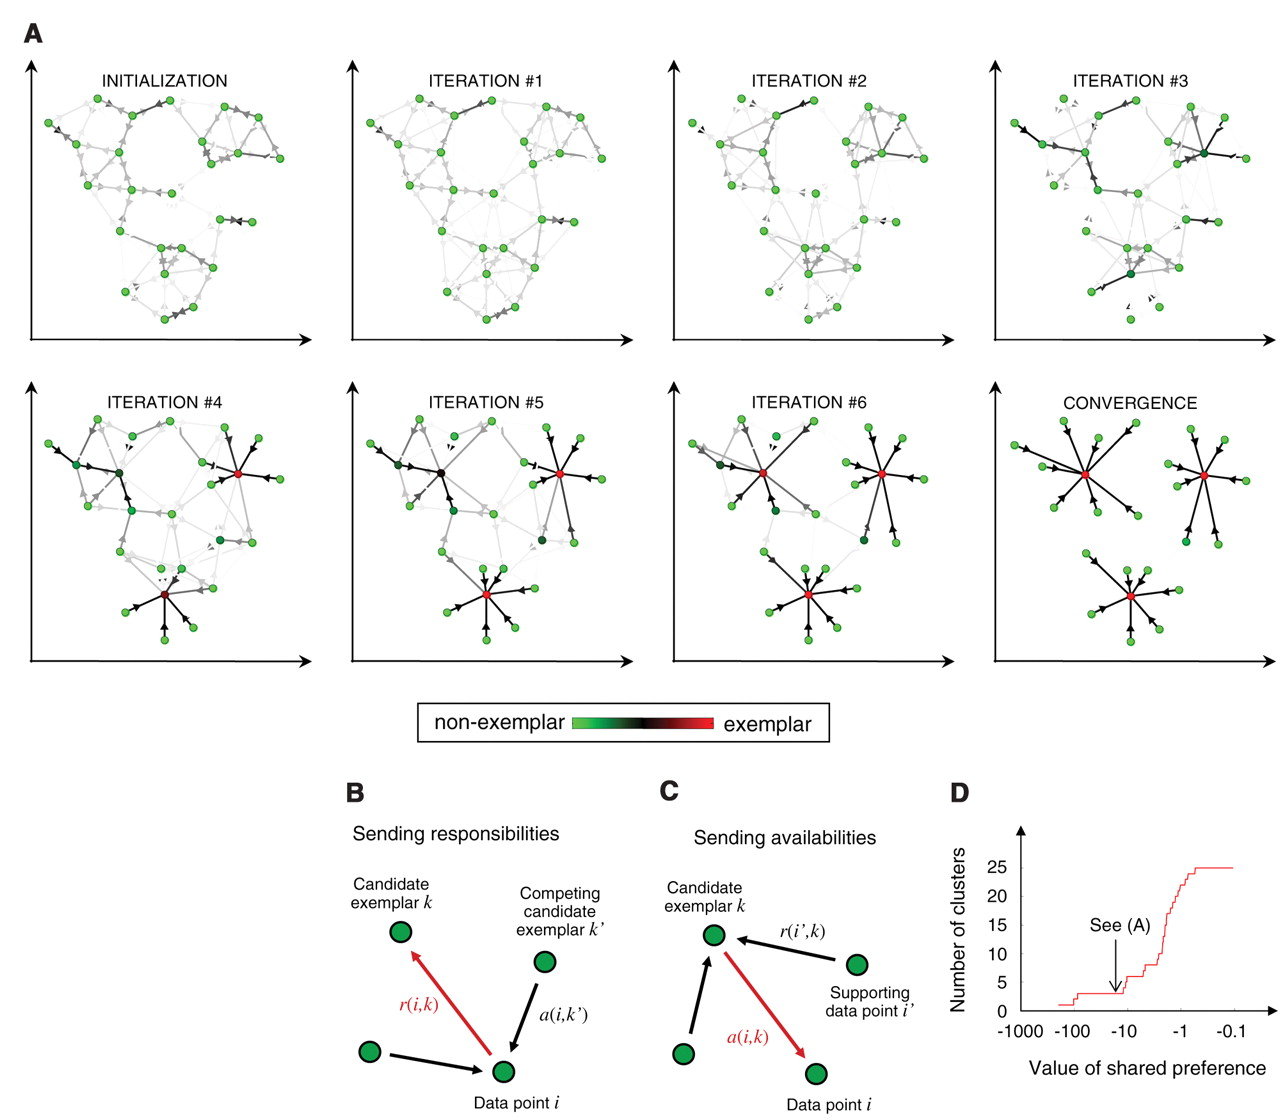
\includegraphics[width=0.7\textwidth]{images/ap.jpg}
\caption{How affinity propagation works}
\label{fig:ap}
\end{figure}

The clustering process described is then applied to the array of similarity calculated previously on features extracted from each words. Once you have run the calculation of clusters, segments are organized into individual folders to provide a visual result of the proceedings just completed. Each group is identified by a segment that represents the centroid of the cluster, which is the element to which all others in the group are closer.
\section{Results}

Let's explore the test phase and see the results in detail. Initially we ran debug tests on our personal PCs in order to easily modify the code, these starting tests and the tests utilized to determine the right value for the many defined constants are not shown here. 

All the tests shown below were performed on a single more powerful machine that has enabled us to work with much larger data in less time. The machine used is composed of two Xeon processors for a total of 16 cores 2.80 Ghz and 48 Gb of RAM.

The tests were performed on a growing number of scans, each containing a maximum of 50 lines from which we extracted the words that represent the states. For each set of scans we present three possible distances calculation: only LCS, only L1 (Euclidean distance) and LCS and L1 combined together through the formula presented in Section 5.

\vspace{3mm}

\begin{itemize}
\item \textbf{Estimated words (E)}: the number of words estimated on the basis of the number of scans(50x).
\item \textbf{Extracted words (W)}: the number of words actually mined and processed, as well as the corresponding percentage.
\item \textbf{Number of clusters (C)}: the number of clusters created in process.
\item \textbf{Running time (T)}: the total execution time, in seconds.
\item \textbf{Average precision (AP)}: the accuracy of the results, the average accuracy of clusters.
$$Precision_{average} = \frac{\sum_i P_i}{N_c}$$
where $P_i$ is the precision of cluster $i$ and $N_c$ is the number of clusters. 
\item \textbf{Precision (P)}: the accuracy of the results, the average accuracy of individual clusters weighted with the number of words.
$$Precision = \frac{\sum_i P_i * n_i}{N_w}$$
where $P_i$ is the precision of cluster $i$, $n_i$ is the number of words in cluster $i$ and $N_w$ is the number of words. 
\end{itemize}

In the next table are shown the main results of the tests. 

\begin{table}[H]
\centering
\footnotesize
\begin{tabular}{|l | c | c | c | c | c | c |} 
 \hline 
 & \textbf{E} &  \textbf{W} & \textbf{C} & \textbf{T} & \textbf{AP} & \textbf{P} \\ [0.5ex] 
 \hline\hline
%% label & estimated words & extracted words & clusters & time & precision %%
16 scans (L1) & 800 & 550 & 55 & 15.52 & 65.06 & 58.00\\ 
16 scans (LCS) & 800 & 550 & 71 & 44.39  & 76.56 & 60.00\\ 
16 scans (LCS and L1) & 800 & 550 & 66 & 47.41 & 74.37 & 62.91\\ \hline
32 scans (L1) & 1600 & 800 & 67 & 38.58 & 59.85 & 52.87\\ 
32 scans (LCS) & 1600 & 800 & 92 & 94.54 & 72.97 & 55.50\\ 
32 scans (LCS and L1) & 1600 & 800 & 86 & 112.90 & 70.19 & 56.25\\ \hline
75 scans (L1) & 3750 & 2350 & 173 & 221.03 & 69.03 & 63.65\\ 
75 scans (LCS) & 3750 & 2350 & 189 & 1169.72 & 75.09 & 67.49\\ 
75 scans (LCS and L1) & 3750 & 2350 & 199 & 1203.28 & 78.01 & 71.16\\ \hline
130 scans (L1) & 6500 & 5050 & 425 & 5444.43 & 76.66 & 71.12\\ 
130 scans (LCS) & 6500 & 5050 & 441 & 5629.71 & 82.11 & 74.41\\ 
130 scans (LCS and L1) & 6500 & 5050 & 463 & 6729.62 & 84.87 & 77.94\\ \hline
500 scans (L1) & 25000 & 18146 & 3957 & 85545.11 & 90.66 & 77.89\\ 
500 scans (LCS) & 25000 & 18146 & 3316 &  76324.63 & 91.02 & 81.22\\ 
500 scans (LCS and L1) & 25000 & 18146 & 3941 & 138309.85\tablefootnote{During this test, the machine used was concurrently executing other tasks creating a bottleneck in the allotted memory, in all similar tests the time was in the order of 90k seconds.} & 92.27 & 82.14\\ 
 \hline
\end{tabular}
\caption{Main results}
\label{table:1}
\end{table}

As we can see in Table \ref{table:1} the number of extracted words is much lower than the estimated number of words. This is mainly due to the fact that not all census tables are completely filled: in some cases there are only a few lines or the states column was purposefully left blank. In other cases the absence of the state samples is due to errors occurring in the segmentation phase due to a wrong interpretation of the rows or the columns.

As we can see in Figure \ref{fig:precision} the accuracy of the cluster grows with the amount of words extracted. This phenomenon is due to the fact that Affinity Propagation works best with a large number of available data: the greater the number of words, the greater the chances of finding words similar between them, and then combine them within a single cluster.


\begin{figure}[H]
\centering
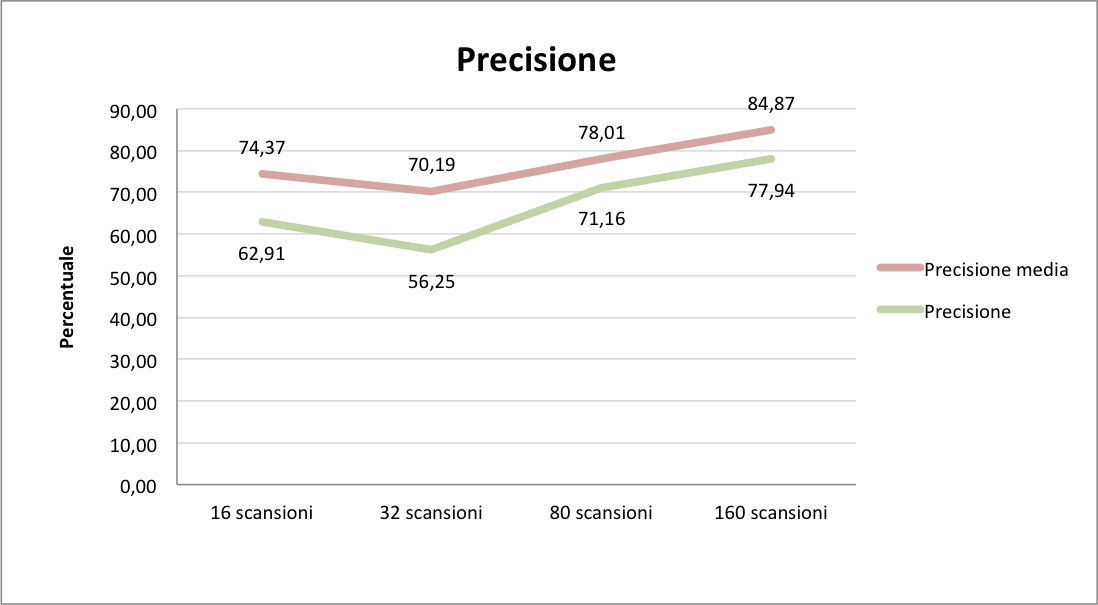
\includegraphics[width=0.7\textwidth]{images/precisione.png}
\caption{Clustering precision relative to the number of scans}
\label{fig:precision}
\end{figure}

In the next table are presented the results regarding the time needed for the calculations. The running time is divided mainly into three distinct categories corresponding to different phases of the process: time needed for the extraction of features, time needed for the creation of similarity matrix (calculation of distances) and time needed for the clustering.

\begin{itemize}
\item \textbf{Features extraction time}: the time, in seconds, required for features extraction from the words.
\item \textbf{Evaluating distances time}: the time, in seconds, required to generate the similarity matrix with the distances between all the words extracted.
\item \textbf{Clustering time}: the time, in seconds, required for the creation of clusters.
\item \textbf{Running time}: the total execution time, in seconds.
\end{itemize}

\begin{table}[H]
\centering
\footnotesize
\begin{tabular}{|l | c | c | c | c |} 
 \hline 
 & \multicolumn{1}{p{2cm}|}{\centering\bfseries Features extraction\\time (s)}&  \multicolumn{1}{p{2cm}|}{\centering\bfseries Evaluating distances\\time (s)} & \multicolumn{1}{p{2cm}|}{\centering\bfseries Clustering\\ time (s)} & \multicolumn{1}{p{2cm}|}{\centering\bfseries Total (s)} \\ [0.5ex] 
 \hline\hline
%% label & features & distances & clusters & total %%
16 scans (L1) & 6.81 & 5.02 & 3.69 & 15.52\\ 
16 scans (LCS) & 6.84 & 34.40 & 3.15 & 44.39\\ 
16 scans (LCS and L1) & 6.84 & 37.32 & 2.85 & 47.41\\ \hline
32 scans (L1) & 11.54 & 7.22 & 19.82 & 38.58\\ 
32 scans (LCS) & 11.27 & 74.72 & 8.55 & 94.54\\ 
32 scans (LCS and L1) & 11.34 & 89.96 & 11.60 & 112.90\\ \hline
75 scans (L1) & 33.65 & 69.00 & 118.38 & 221.03\\ 
75 scans (LCS) & 35.13 & 1002.63 & 131.96 & 1169.72\\ 
75 scans (LCS and L1) & 34.70 & 1070.92 & 97.66 & 1203.28\\ \hline
130 scans (L1) & 70.80 & 313.70 & 5059.93 & 5444.43\\ 
130 scans (LCS) & 68.17 & 4353.85 & 1207.69 & 5629.71\\ 
130 scans (LCS and L1) & 73.10 & 5608.82 & 1047.70 & 6729.62\\ \hline
500 scans (L1) & 289.33 & 4482.02 & 80773.76 & 85545.11 \\ 
500 scans (LCS) & 323.66 & 57699.51 & 18301.46 & 76324.63\\ 
500 scans (LCS and L1) & 403.41 & 61424.57 & $76481.87^5$ & $138309.85^5$\\ 
 \hline
\end{tabular}
\caption{Running time}
\label{table:2}
\end{table}

As we can see in Table \ref{table:2} the complexity is mainly due to the construction phase of the similarity matrix, that is the calculation of distances. This high operative cost occurs especially in calculating the LCS distance due to the fact that the structural strings of our words are very long and the cost of the algorithm is $O(nm)$, with $n$ and $m$ the lengths of the two strings, cost that must be considered in each comparison between couples of samples.

We sought long structural strings to obtain a deeper characterization of the words (and therefore make more accurate clustering), but this necessarily increases the calculation time.

\begin{figure}[!htbp]
\centering
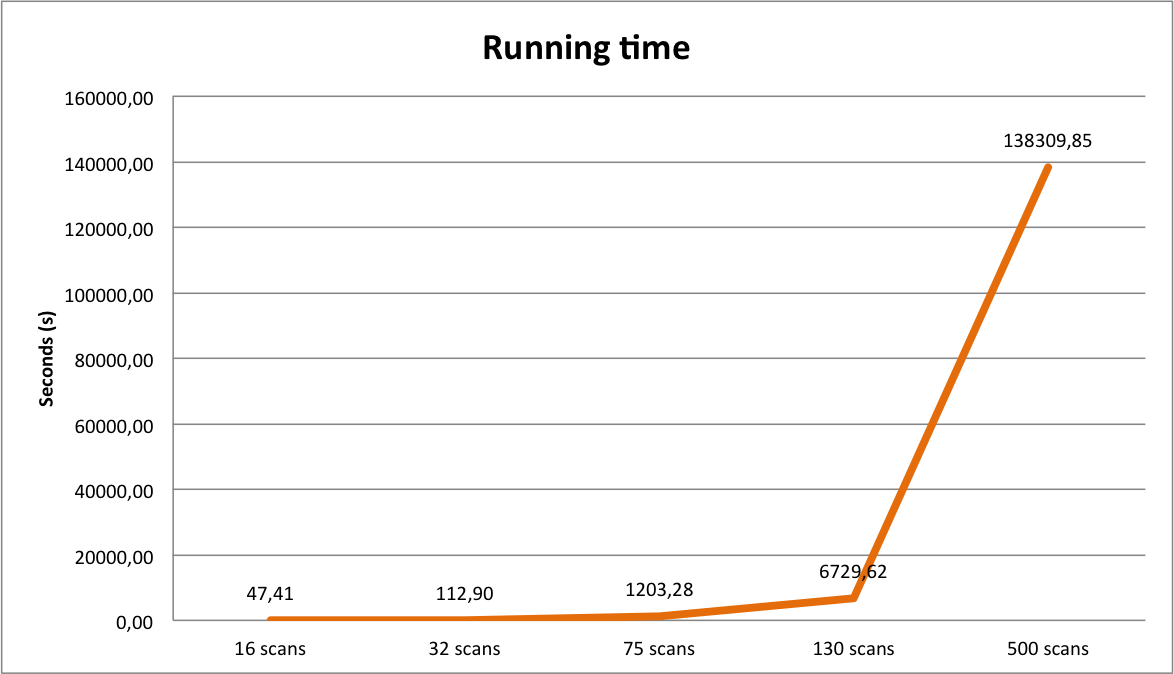
\includegraphics[width=0.7\textwidth]{images/esecuzione}
\caption{Running time relative to the number of scans}
\label{fig:time}
\end{figure}

A parameter to evaluate the goodness of our application relatively to the task can be the number of clusters that have the absolute precision, that is contain only similar elements that are properly classified(due to human error sometimes the words in the debug files suffer a faulty categorization).

In the following table are presented the number of clusters which respect the above property and the number of items that they contain. 

\begin{itemize}

\item \textbf{Correct clusters}: the number of clusters with absolute precision, therefore containing only words equal to each other.
\item \textbf{Correct words}: the number of words within the Correct clusters and their corresponding percentage respect to all the elements.
\item \textbf{Single clusters}: clusters containing only one word.
\item \textbf{Average words for correct non-single cluster} (\textbf{AWCC}): number of words in average in the correct clusters that do not contain a single element.
\end{itemize}

\begin{table}[H]
\centering
\footnotesize
\begin{tabular}{|l | c | c | c | c |} 
 \hline 
 & \multicolumn{1}{p{2cm}|}{\centering\bfseries Correct\\ clusters}&  \multicolumn{1}{p{2cm}|}{\centering\bfseries Correct\\words} & \multicolumn{1}{p{2cm}|}{\centering\bfseries Single\\clusters} & \multicolumn{1}{p{2cm}|}{\centering\bfseries AWCC} \\ [0.5ex] 
 \hline\hline
%% label & clusters & words & percentage %%
16 scans (L1) & 12 & 18 & 10 &  3.00\\ 
16 scans (LCS) & 33 & 44 & 29 & 2.75\\ 
16 scans (LCS and L1) & 25 & 45 & 18 & 6.43\\ \hline >>>CONTINUAMI
32 scans (L1) & 11 & 11 & 10 & xx.00\\ 
32 scans (LCS) & 39 & 48 & 36 &1.23\\ 
32 scans (LCS and L1) & 32 & 43 & 28 & 1.34\\ \hline
75 scans (L1) & 39 & 172 & 11 & 4.41\\ 
75 scans (LCS) & 78 & 265 & 43 & 3.40\\ 
75 scans (LCS and L1) & 77 & 316 & 43 & 4.10\\ \hline
130 scans (L1) & 138 & 651 & 23 & 4.72\\ 
130 scans (LCS) & 208 & 713 & 107 &  3.43\\ 
130 scans (LCS and L1) & 215 & 860 & 89 & 4.00\\ \hline
500 scans (L1) & 2854 & 7354 & 151 & 2.58\\ 
500 scans (LCS) & 2902 & 7423 & 163 & 2.56\\ 
500 scans (LCS and L1) & 3020 & 7616 & 145 & 2.52\\ 
 \hline
\end{tabular}
\caption{Correct clusters}
\label{table:3}
\end{table}

\section{Compiling and running notes}

This software was developed entirely in C++, and uses an open source library of image processing and analysis, \emph{Leptonica}\footnote{Leptonica,a pedagogically-oriented open source site containing software that is broadly useful for image processing and image analysis applications -http://www.leptonica.org/}, version 1.70.

\emph{Leptonica} provides many functions for manipulating images pixel by pixel using a high-level approach. Thanks to this library for example, you can draw up a diagram of projections, crop images, or find the connected components in a portion of the image.

To compile the code, once included the library described above, it is necessary, in the case of version of \emph{GCC/G++} less than 4.7, compile with version 11 of C++ that introduces support for threads.

To run this programm use the following parameters:
\begin{itemize}
\item \textbf{-d} to specify the images directory.
\item \textbf{-t} to specify the number of threads. Default is 2.
\item \textbf{-\--lcs} to use only LCS distance for building similarity matrix.
\item \textbf{-\--l1} to use only Euclidean distance for building similarity matrix.
\end{itemize}
\section{Conclusion}

Based on the results obtained we can note that the accuracy of the cluster grows with the amount of words extracted. This phenomenon is due to the fact that Affinity Propagation works best with a large number of available data: the greater the number of words, the greater the chances of finding words similar between them, and then combine them within a single cluster.

We can see then that, with the increase of the processed words, correct clusters also increase. This result enables to divide with a good approximation the words between them, even bringing the cluster that contains the same words in post processing.

The other factor to consider is the weather: as shown by the graph above the time increases nearly exponentially as a function of the number of words you want to extract. This, as shown, is due at the time of calculation of the distances between the structural strings of word with LCS. Using another calculation method you might reduce the necessary computing time .

\begin{thebibliography}{1}

\bibitem{vecchioBib}
Alessio Melani, Moreno Niccolai, \emph{Segmentazione e Clustering di Stati del censimento americano del 1940}.\hskip 1em plus
  0.5em minus 0.4em\relax Database Technology course, University of Florence, 2014.

\bibitem{clustBib}
Brendan J. Frey, Delbert Dueck, \emph{Clustering by Passing Messages
Between Data Points}.\hskip 1em plus
  0.5em minus 0.4em\relax http://www.sciencemag.org/, 2007.


\end{thebibliography}



\end{document}